\section{Architecture Integration}

\subsection{Model Support}

\begin{table}[H]
\centering
\small
\begin{tabular}{llllll}
\toprule
\textbf{Architecture} & \textbf{Attention} & \textbf{Nested?} & \textbf{RoPE?} & \textbf{GQA?} & \textbf{Cross-attn?} \\
\midrule
DistilBERT & Flat & No & No & No & No \\
RoBERTa & Nested & Yes & No & No & No \\
GPT-2 & Causal & No & No & No & No \\
Qwen3.5 & GQA+RoPE & No & Yes & Yes & No \\
T5 & Enc-Dec & No & No & No & Yes \\
\bottomrule
\end{tabular}
\end{table}

\subsection{Weight Extraction}

\subsubsection{DistilBERT (Flat)}
\begin{lstlisting}
q\_w = src.q\_lin.weight
k\_w = src.k\_lin.weight
v\_w = src.v\_lin.weight
o\_w = src.out\_lin.weight
\end{lstlisting}

\subsubsection{RoBERTa (Nested)}
\begin{lstlisting}
q\_w = src.self.query.weight
k\_w = src.self.key.weight
v\_w = src.self.value.weight
o\_w = src.output.dense.weight
is\_nested\_encoder = True
\end{lstlisting}

\subsubsection{GPT-2 (Conv1D)}
\begin{lstlisting}
w = src.c\_attn.weight.T
q\_w, k\_w, v\_w = w.chunk(3, dim=0)
o\_w = src.c\_proj.weight.T
\end{lstlisting}

\subsubsection{Qwen (GQA + RoPE)}
Direct copy with GQA-aware dims.

\subsection{Injection}

\begin{lstlisting}
def inject\_fusion\_attn(layer, cfg, comp\_config, old\_attn):
    new = FUSIONATTN(
        config=cfg,
        comp\_config=comp\_config,
        old\_attn=old\_attn,
        block\_size=64,
        top\_k\_blocks=4,
    )
    if hasattr(layer, "attention"):
        if hasattr(layer.attention, "self"):
            layer.attention.self = new
        else:
            layer.attention = new
    return new
\end{lstlisting}

\subsection{Nested Encoder Bypass}

For RoBERTa, \texttt{out\_proj} is not applied; outer \texttt{BertSelfOutput.dense} does it.

\subsection{GQA}

\begin{lstlisting}
if self.kv\_repeat \textgreater{} 1:
    k = repeat\_kv(k, self.kv\_repeat)
    v = repeat\_kv(v, self.kv\_repeat)
\end{lstlisting}

\subsection{RoPE}

Supports partial RoPE (Qwen3.5 with rotary\_dim \textless{} head\_dim).

\subsection{Registry}

\begin{lstlisting}
@ATTENTION\_REGISTRY.register("fusion\_attn")
class FUSIONATTN(BaseAttention):
    ...
\end{lstlisting}

\subsection{Failure Modes}

\begin{table}[H]
\centering
\small
\begin{tabular}{lll}
\toprule
\textbf{Failure} & \textbf{Detection} & \textbf{Response} \\
\midrule
Missing weights & Frobenius \textless{} 1e-4 & \textbf{raise RuntimeError} \\
Zero Frobenius & Same & \textbf{raise RuntimeError} \\
Empty blocks & Padding mask & -inf \\
NaN in scores & nan\_to\_num & Replace 0 \\
\bottomrule
\end{tabular}
\end{table}

\textbf{   Critical:} \texttt{inject\_fusion\_attn} has \texttt{raise RuntimeError("copy\_weights failed")} 
which kills the injection on any failure. Recommend changing to \texttt{return None}.

\subsection{Numerical Stability}

\begin{table}[H]
\centering
\small
\begin{tabular}{ll}
\toprule
\textbf{Component} & \textbf{Precision} \\
\midrule
Base weights & Model dtype \\
LoRA & Model dtype \\
Gate MLP & Model dtype \\
Attention scores & FP32 \\
Softmax & FP32 \\
Output & Model dtype \\
\bottomrule
\end{tabular}
\end{table}



\begin{figure}[H]
\centering
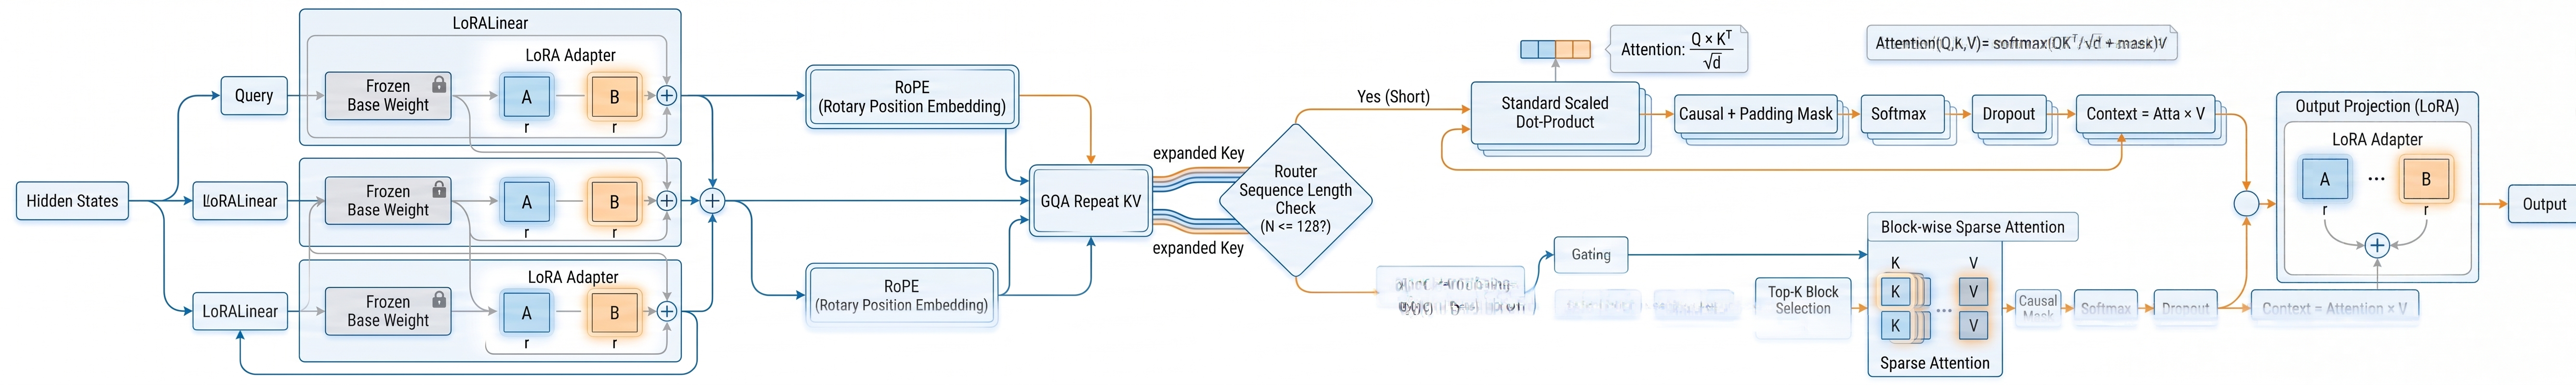
\includegraphics[width=\linewidth]{figures/architecture.jpeg}
\caption{High-level architectural diagram of fusion.}
\label{fig:arch_fusion}
\end{figure}

